% Generated by code/scripts/report_figures.py at 2026-11-06T09:28:43Z; do not edit.
% Inputs: artifacts/cluster/runs/bench16-20261105T092045Z-1523703
\begin{figure}[t]
\centering
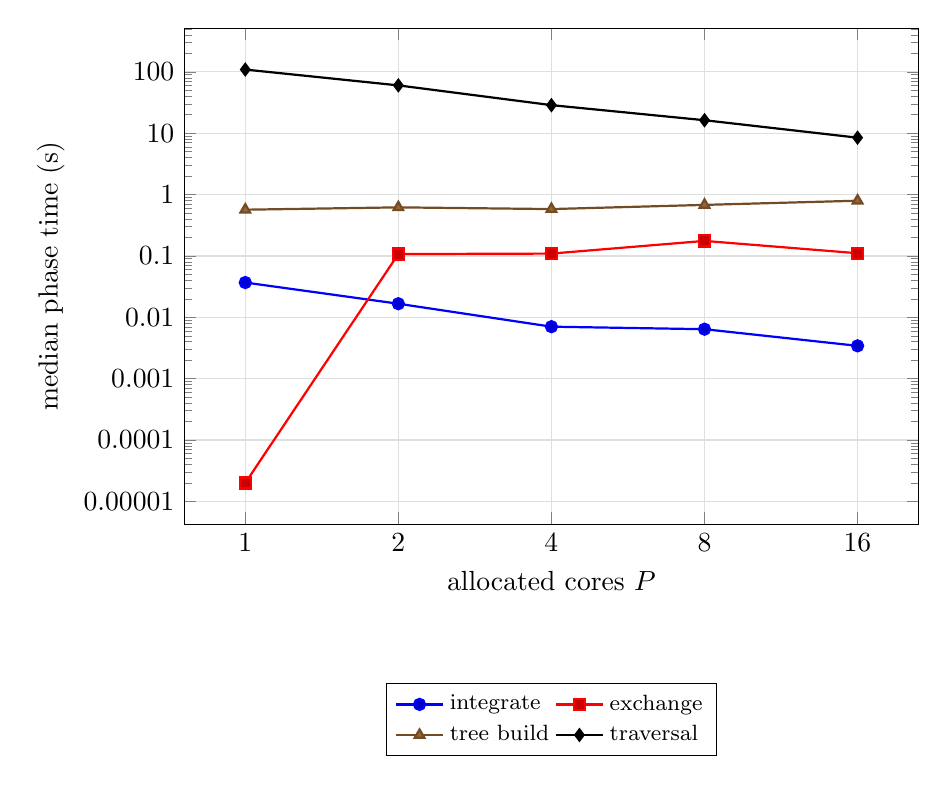
\begin{tikzpicture}
\begin{axis}[width=0.9\columnwidth, height=0.65\columnwidth, xlabel={allocated cores $P$}, ylabel={median phase time (s)}, xmode=log, log basis x=2, log ticks with fixed point, ymode=log, ytick={1e-05,0.0001,0.001,0.01,0.1,1,10,100,1000}, legend style={at={(0.5,-0.32)}, anchor=north, legend columns=2, font=\footnotesize}, legend cell align=left, grid=major, grid style={gray!25}]
\addplot+[mark=*, thick] coordinates {(1,0.03688) (2,0.01665) (4,0.007037) (8,0.006403) (16,0.00343)};
\addlegendentry{integrate}
\addplot+[mark=square*, thick] coordinates {(1,2e-05) (2,0.1073) (4,0.1093) (8,0.1759) (16,0.1107)};
\addlegendentry{exchange}
\addplot+[mark=triangle*, thick] coordinates {(1,0.5671) (2,0.6192) (4,0.5808) (8,0.6794) (16,0.7948)};
\addlegendentry{tree build}
\addplot+[mark=diamond*, thick] coordinates {(1,109) (2,60.2) (4,28.69) (8,16.29) (16,8.458)};
\addlegendentry{traversal}
\end{axis}
\end{tikzpicture}
\caption{Phase times of the strong-scaling runs with $T=1$. Each phase is the maximum over ranks, so the phases need not sum to the wall time; zero values are omitted from the log axis. Vanda job 1523703: 16 cores of a shared Gold 6438N node, 3 interleaved repetitions.}
\label{fig:phases}
\end{figure}
